% ___________________________________________
    % Questionnaire usagers
    %\newpage
    \setcounter{section}{0}
\chapterheader{Annexes sur le questionnaire auprès des usager·ère·s}
\chapter{Annexes liées à la mise en œuvre du questionnaire auprès des usager·ère·s}
    \label{annexes:questionnaire-usagers}

    % Renvoi
L'\hyperref[annexes:questionnaire-usagers]{annexe~\ref{annexes:questionnaire-usagers}} se réfère à la \hyperref[chap3:questionnaire]{section consacrée à l'enquête par questionnaire sur les pratiques intermodales} (page \pageref{chap3:questionnaire}), dans le cadre du \hyperref[chap3:titre]{chapitre~3} (page \pageref{chap3:titre}), et veille à fournir des informations supplémentaires sur le protocole méthodologique du questionnaire conduit auprès des usager·ère·s.%%Rédigé%%

    % ___________________________________________
    % Mini-sommaire
    \setcounter{tocdepth}{2}
    % Redéfinir le titre de la table des matières locale
    \renewcommand{\localcontentsname}{Structure de l'annexe~\ref{annexes:questionnaire-usagers}}
\localtableofcontents

    % Affiche questionnaire en anglais
    \newpage
    \needspace{1\baselineskip} % Réserve de l'espace
    \sectionheader{Affiche du questionnaire}
\section{Affiche du questionnaire auprès des usager·ère·s (anglais)}
    \label{annexes:affiche-en-questionnaire-usagers}

    % Affiche questionnaire anglais
    \begin{figure}[H]\vspace*{4pt}
        \caption*{}
        \centerline{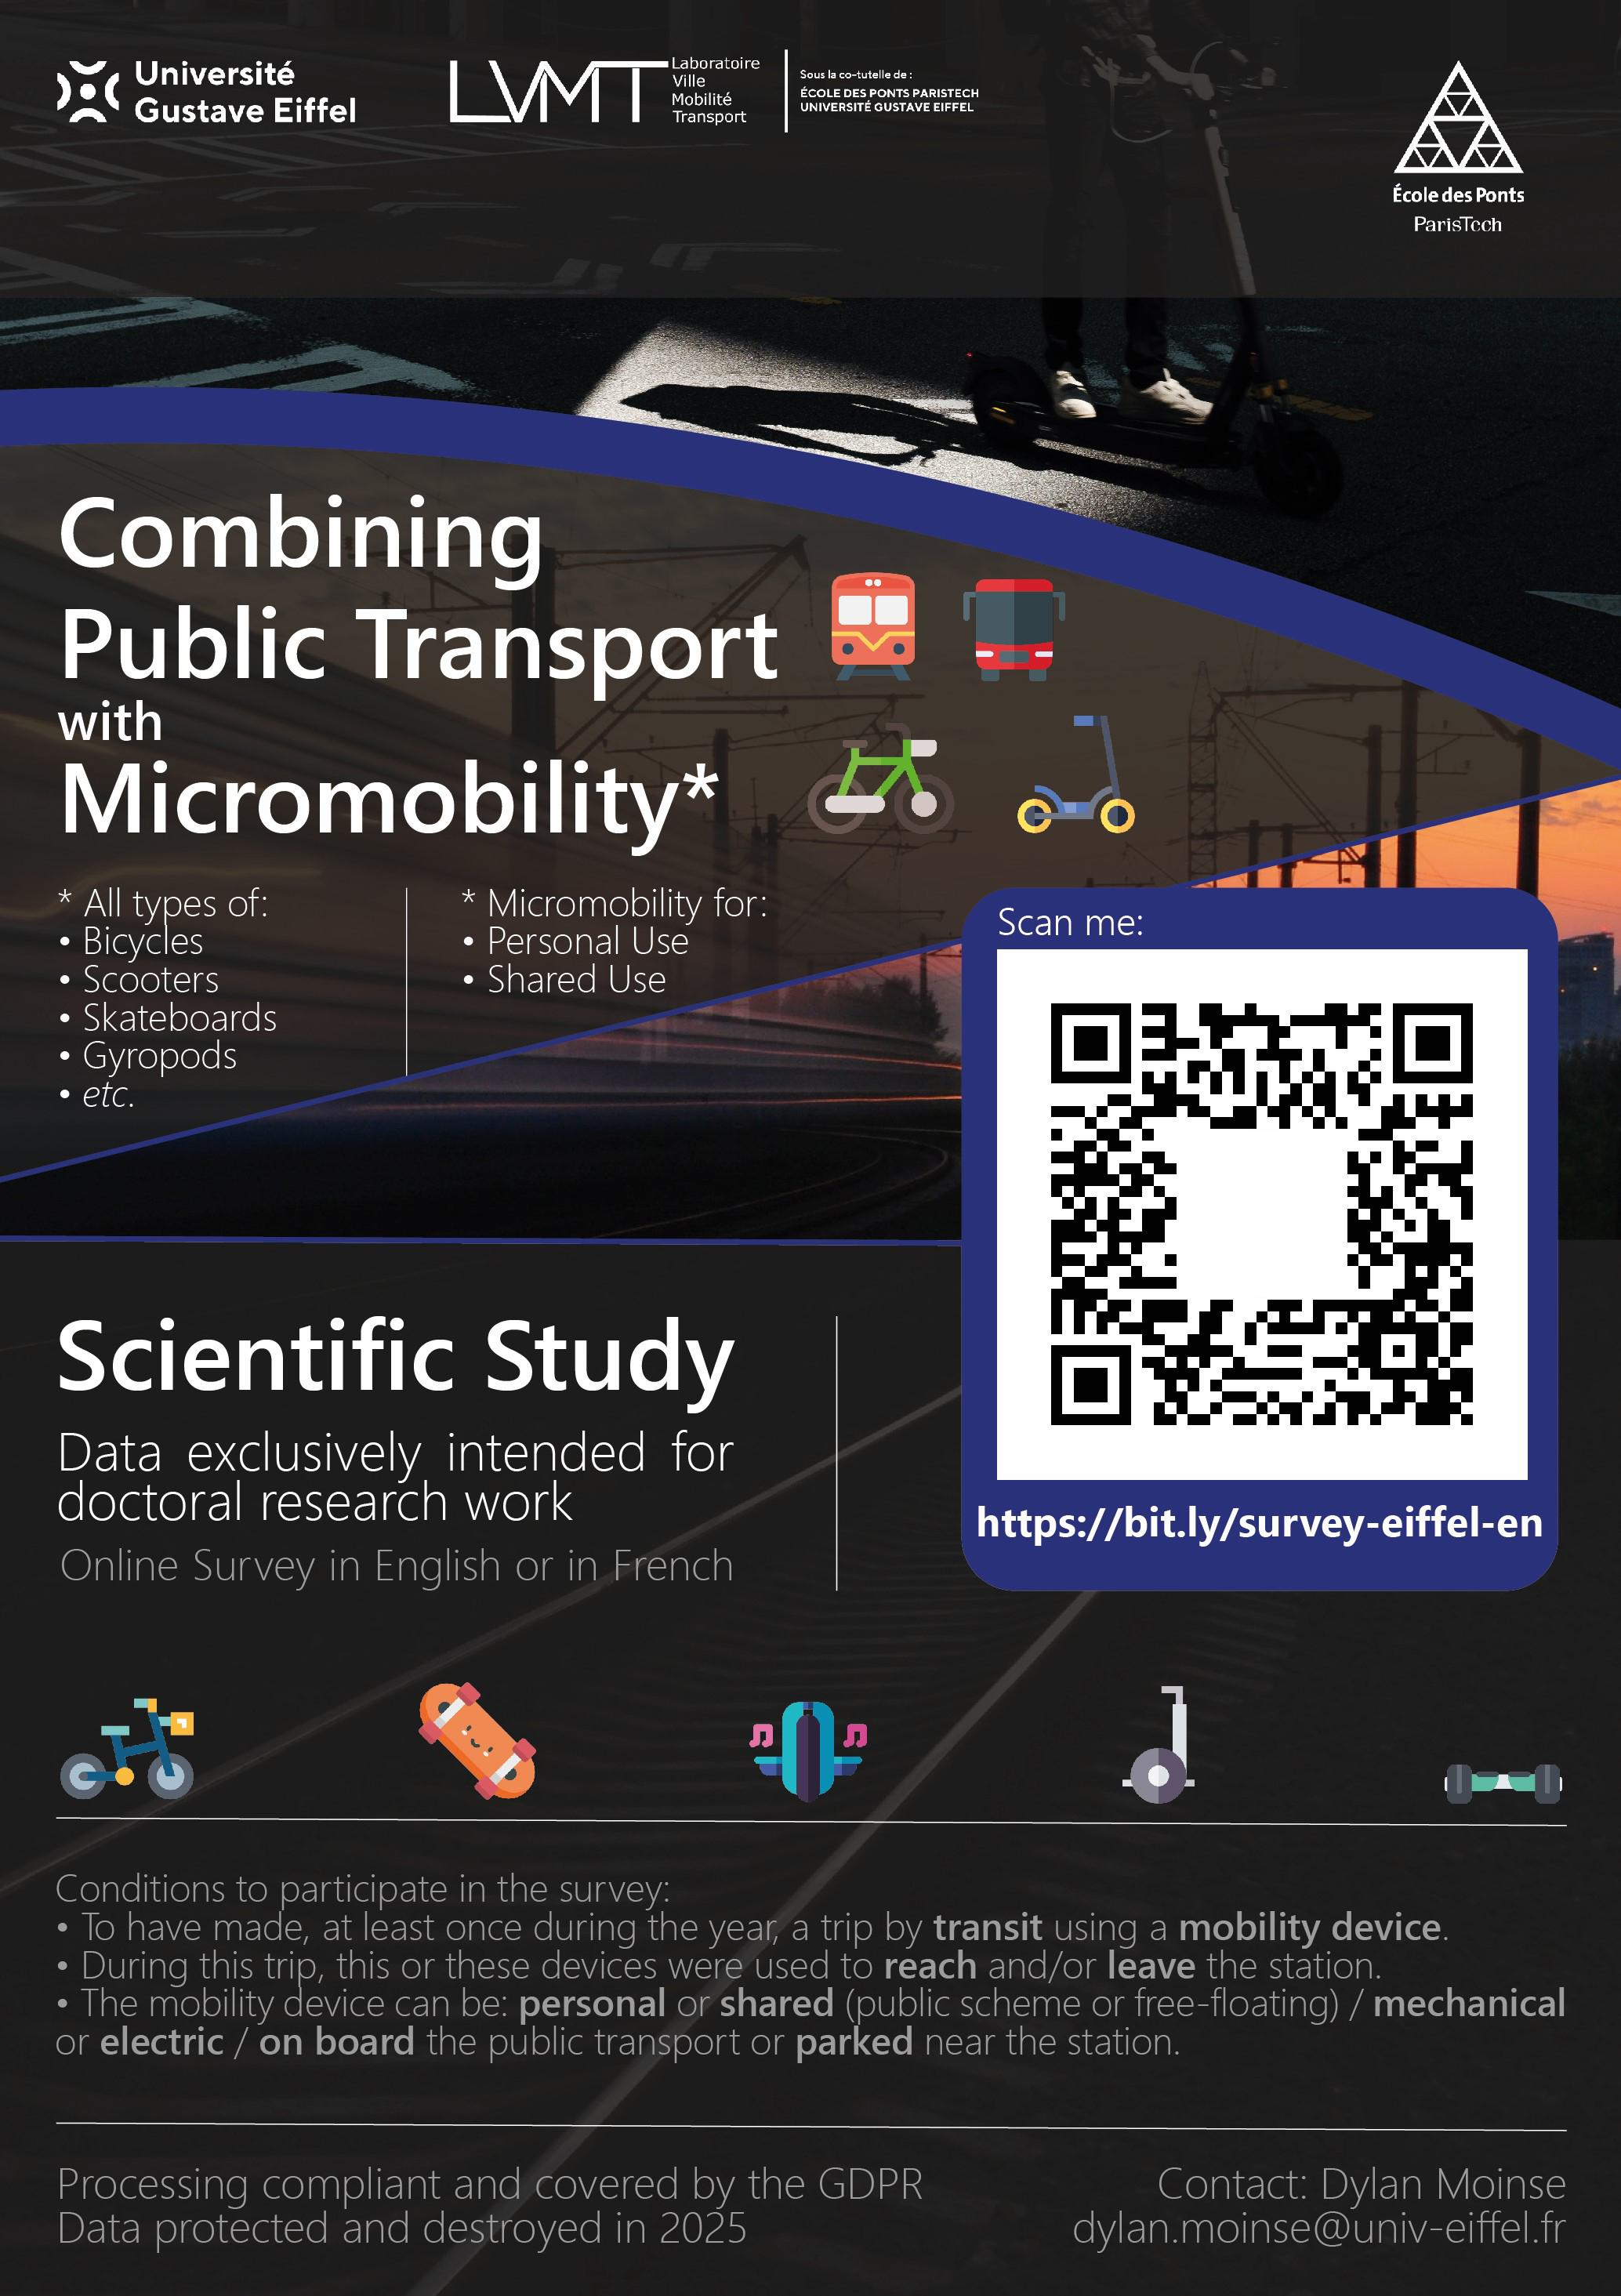
\includegraphics[width=1\columnwidth]{src/Figures/Annexes/EN_Affiche_questionnaire.jpg}}
        \vspace{5pt}
        \begin{flushright}\scriptsize{
        Auteur~: \textcolor{blue}{Dylan Moinse (2021)}
        }\end{flushright}
    \end{figure}

    \newpage
    % Structure questionnaire
    \newpage
    \needspace{1\baselineskip} % Réserve de l'espace
    \sectionheader{Structure du questionnaire}
\section{Structure du questionnaire auprès des usager·ère·s}
    \label{annexes:structure-questionnaire-usagers}

\textbf{Étude sur la Combinaison du Vélo et de la Micro-mobilité avec les Transports en Commun}

\textsl{Vous êtes invité·e à participer à un projet de recherche portant sur l'usage des transports en commun en lien avec le vélo ou les options de micro-mobilité. L'enquête vise à mieux comprendre les mécanismes et les enjeux de ce phénomène de mobilité croissant, sous l'angle de la mobilité et de l'urbanisme, dans l'intérêt de proposer des solutions aux usager·ère·s.}%%Rédigé%%

\textsl{Pour contribuer à cette enquête, il est nécessaire de remplir la condition suivante~: avoir réalisé un déplacement combinant un mode de déplacement léger (vélo, trottinette, \textsl{etc}.) avec un mode de transport en commun (train, métro, \textsl{etc}.). Par modes de déplacement légers, nous entendons le vélo, la trottinette électrique ou bien d'autres engins de déplacement, qu'ils soient personnels ou partagés (vélo ou trottinette en libre-service ou en \textsl{free-floating}, \textsl{etc}.) et embarqués à bord des transports en commun ou bien stationnés ou déposés pendant le voyage.}%%Rédigé%%

\textsl{Ce questionnaire dure environ vingt minutes.}%%Rédigé%%

\textsl{Cette étude s'inscrit dans le cadre d'une thèse de doctorat au Laboratoire Ville Mobilité Transport (Université Gustave Eiffel et École des Ponts).}%%Rédigé%%

\textsl{En conformité avec le \acrfull{RGPD}, les données recueillies dans le présent formulaire sont anonymisées et seront traitées exclusivement dans le cadre de cette mission de recherche, à savoir la collecte des représentations sociales et la spatialisation de ces déplacements intermodaux. D'une durée approximative de vingt minutes, il vous est possible d'interrompre l'enquête à tout moment. Il convient également d'indiquer que \Marque{LimeSurvey} est un outil promu par les universités françaises et compatible avec la protection des données à caractère personnel.}%%Rédigé%%

\textsl{En choisissant de participer à cette enquête~:
\begin{customitemize}
    \item Vous déclarez que votre participation est volontaire et vous pourrez, à tout moment, interrompre cette démarche, sans avoir à vous justifier~;
    \item Vous pourrez prendre connaissance des résultats de l'étude dans sa globalité lorsqu'elle sera achevée~;
    \item Les données recueillies demeureront strictement confidentielles.
\end{customitemize}}%%Rédigé%%

\textsl{La réglementation en matière d'utilisation des données personnelles à l'Université Gustave Eiffel est conforme à la loi Informatique et Libertés du 6 janvier 1978 modifiée et au Règlement UE 2016/679 du Parlement européen et du Conseil du 27 avril 2016, relatif à la protection des personnes physiques à l'égard du traitement des données à caractère personnel et à la libre circulation de ces données.}%%Rédigé%%

\textsl{Seul l'enquêteur a accès aux données qui seront conservées pendant cinq ans. Vous avez le droit de contacter les \acrfull{DPO} de l’Université Gustave Eiffel ou saisir la \acrfull{CNIL}.}%%Rédigé%%

\textsl{Nous vous remercions sincèrement de votre participation et de votre intérêt.}%%Rédigé%%

    % Tableau structure du questionnaire usagers
% Tableau T1
%%Rédigé%%
  \begin{table}[h!]
    \centering
    \renewcommand{\arraystretch}{1.5}
    \resizebox{\columnwidth}{!}{
    \begin{tabular}{p{0.1\columnwidth}p{0.6\columnwidth}p{0.15\columnwidth}p{0.15\columnwidth}}
      % \hline
      \rule{0pt}{15pt} \textcolor{blue}{\textbf{\small{\(T_{1}\)}}} & \textcolor{blue}{\textbf{\small{Intitulé de la question}}} & \textcolor{blue}{\textbf{\small{Type}}} & \textcolor{blue}{\textbf{\small{Réponses}}}\\
      \hline
\multicolumn{4}{l}{\textbf{Consentement}}\\
    \small{\textbf{\(Q_{01}^{T_{1}}*\)}} & \small{\textsl{Compte tenu des informations qui m’ont été transmises, j’accepte librement de participer à ce questionnaire de recherche.}} & \small{Choix unique} & \small{Oui~| Non}\\
      \hline
    \end{tabular}}
    \caption*{}
    \vspace{5pt}
        \end{table}

% Tableau T2
%%Rédigé%%
  \begin{table}[h!]
    \centering
    \renewcommand{\arraystretch}{1.5}
    \resizebox{\columnwidth}{!}{
    \begin{tabular}{p{0.1\columnwidth}p{0.35\columnwidth}p{0.15\columnwidth}p{0.5\columnwidth}}
      % \hline
      \rule{0pt}{15pt} \textcolor{blue}{\textbf{\small{\(T_{2}\)}}} & \textcolor{blue}{\textbf{\small{Intitulé de la question}}} & \textcolor{blue}{\textbf{\small{Type}}} & \textcolor{blue}{\textbf{\small{Réponses}}}\\
      \hline
\multicolumn{4}{l}{\textbf{Déplacement intermodal}}\\
    \small{\textbf{\(Q_{01}^{T_{2}}*\)}} & \small{\textsl{Quel(s) mode(s) de transport en commun avez-vous emprunté lors de votre dernier déplacement intégrant l'utilisation d'un vélo ou d'une option de micro-mobilité~?}} & \small{Choix multiples} & \small{TGV~| TERGV~| TER~| RER~| Métro~| Tramway~| Bus~| \textsl{\textsl{Autre(s)}}}\\
\hline
    \small{\textbf{\(Q_{02}^{T_{2}}*\)}} & \small{\textsl{Quelles sont les stations de départ et d'arrivée (et de correspondance) de ce déplacement réalisé en transport en commun~?}} & \small{Textuel} & \small{\textsl{Nom de la station de départ}~| \textsl{Nom de la station de destination}~| \textsl{Nom des stations en correspondance}}\\
\hline
    \small{\textbf{\(Q_{03}^{T_{2}}*\)}} & \small{\textsl{De quelle manière vous êtes-vous rendu·e à partir du lieu d'origine (votre domicile, le cas échéant) jusqu'à \textcolor{blue}{station de départ}~?}} & \small{Choix multiples} & \small{Marche~| Vélo ou micro-mobilité~| Transports en commun urbains~| Voiture (conducteur·rice)~| Voiture (passager·ère)~| Taxi ou VTC~| Scooter ou moto~| Autopartage~| \textsl{Autre(s)}}\\
\hline
    \small{\textbf{\(Q_{04}^{T_{2}}*\)}} & \small{\textsl{Comment évaluez-vous le confort et la qualité de ce segment de trajet allant du lieu d'origine à \textcolor{blue}{station de départ}~?}} & \small{Choix unique} & \small{Très positifs~| Positifs~| Relativement positifs~| Relativement négatifs~| Négatifs~| Très négatifs~| Je ne sais pas}\\
\hline
    \small{\textbf{\(Q_{05}^{T_{2}}*\)}} & \small{\textsl{De quelle manière vous êtes-vous rendu·e de \textcolor{blue}{station d'arrivée} jusqu'à \textcolor{blue}{lieu de destination}~?}} & \small{Choix multiples} & \small{Marche~| Mode de déplacement léger~| Transports en commun urbains~| Voiture (conducteur·rice)~| Voiture (passager·ère)~| Taxi ou VTC~| Scooter ou moto~| Autopartage~| \textsl{Autre(s)}}\\
\hline
    \small{\textbf{\(Q_{06}^{T_{2}}*\)}} & \small{\textsl{Comment évaluez-vous le confort et la qualité de ce segment de trajet allant de \textcolor{blue}{station d'arrivée} à votre lieu de destination~?}} & \small{Choix unique} & \small{Très positifs~| Positifs~| Relativement positifs~| Relativement négatifs~| Négatifs~| Très négatifs~| Je ne sais pas}\\
\hline
    \small{\textbf{\(Q_{07}^{T_{2}}*\)}} & \small{\textsl{À quel(s) type(s) de vélo ou de micro-mobilité avez-vous eu recours lors de ce déplacement combiné avec le(s) \textcolor{blue}{mode(s) de transport en commun~?}}} & \small{Choix multiples} & \small{Vélo classique~| Vélo pliant~| Trottinette~| Skateboard~| Gyroroue ou Monoroue~| Hoverboard~| Gyropode ou Segway~| \textsl{Autre(s)}}\\
\hline
    \small{\textbf{\(Q_{08}^{T_{2}}*\)}} & \small{\textsl{Votre (vos) \textcolor{blue}{mode(s) de déplacement} est-il (sont-ils) électrique(s)~?}} & \small{Choix unique} & \small{Oui~| Non~| Je ne sais pas~| \textsl{Autre(s)}}\\
\hline
    \small{\textbf{\(Q_{09}^{T_{2}}*\)}} & \small{\textsl{Possédez-vous votre (vos) \textcolor{blue}{mobilité individuelle légère}~?}} & \small{Choix multiples} & \small{Oui, je le(s) possède~| Non, je me sers d'un système de location longue durée~| Non, je me sers d'un service en libre-service~| Non, c'est un véhicule de fonction (professionnel)~| Non, je l'(les) emprunte auprès de pairs (famille, amis, \textsl{etc}.)~| \textsl{Autre(s)}}\\
\hline
    \small{\textbf{\(Q_{10}^{T_{2}}*\)}} & \small{\textsl{Depuis combien de temps avez-vous recours à cette combinaison en \textcolor{blue}{mobilité individuelle légère} et en \textcolor{blue}{mode(s) de transport en commun}~?}} & \small{Choix multiples} & \small{Depuis plusieurs années~| Depuis un an environ~| Depuis quelques mois~| Depuis moins d'un mois~| C'était la première fois~| Je ne sais pas~| \textsl{Autre(s)}}\\
\hline
    \small{\textbf{\(Q_{+}^{T_{2}}\)}} & \small{Champ d'expression libre} & \small{Textuel} & \small{-}\\
      \hline
    \end{tabular}}
    \caption*{}
    \vspace{5pt}
        \end{table}

% Tableau T3
%%Rédigé%%
  \begin{table}[h!]
    \centering
    \renewcommand{\arraystretch}{1.5}
    \resizebox{\columnwidth}{!}{
    \begin{tabular}{p{0.1\columnwidth}p{0.35\columnwidth}p{0.15\columnwidth}p{0.5\columnwidth}}
      % \hline
      \rule{0pt}{15pt} \textcolor{blue}{\textbf{\small{\(T_{3}\)}}} & \textcolor{blue}{\textbf{\small{Intitulé de la question}}} & \textcolor{blue}{\textbf{\small{Type}}} & \textcolor{blue}{\textbf{\small{Réponses}}}\\
      \hline
\multicolumn{4}{l}{\textbf{Points de repère géographiques}}\\
    \small{\textbf{\(Q_{01}^{T_{3}}*\)}} & \small{\textsl{Quel est l'emplacement du lieu de départ (votre domicile, le cas échéant) de ce déplacement effectué en \textcolor{blue}{mobilité individuelle légère} et en \textcolor{blue}{mode(s) de transport en commun}~?}} & \small{Textuel} & \small{Numéro de voie~| Voie~| Commune~| Code postal~| Pays}\\
\hline
    \small{\textbf{\(Q_{02}^{T_{3}}*\)}} & \small{\textsl{Localisez le lieu de départ de ce déplacement sur la carte.}} & \small{Carte interactive} & \small{-}\\
\hline
    \small{\textbf{\(Q_{03}^{T_{3}}*\)}} & \small{\textsl{Lors de ce trajet de \textcolor{blue}{lieu d'origine} à \textcolor{blue}{station de départ}, avez-vous pris le chemin le plus court possible~?}} & \small{Choix unique} & \small{Oui~| Non~| Je ne sais pas~| \textsl{Autre(s)}}\\
\hline
    \small{\textbf{\(Q_{04}^{T_{3}}*\)}} & \small{\textsl{Quel est l'emplacement du lieu de destination de ce déplacement effectué en \textcolor{blue}{mobilité individuelle légère} et en \textcolor{blue}{mode(s) de transport en commun}~?}} & \small{Textuel} & \small{Numéro de voie~| Voie~| Commune~| Code postal~| Pays}\\
\hline
    \small{\textbf{\(Q_{05}^{T_{3}}*\)}} & \small{\textsl{Localisez le lieu de destination de ce déplacement sur la carte.}} & \small{Carte interactive} & \small{-}\\
\hline
    \small{\textbf{\(Q_{06}^{T_{3}}*\)}} & \small{\textsl{Lors de ce trajet de \textcolor{blue}{station d'arrivée} à \textcolor{blue}{lieu de destination}, avez-vous pris le chemin le plus court possible~?}} & \small{Choix unique} & \small{Oui~| Non~| Je ne sais pas~| \textsl{Autre(s)}}\\
\hline
    \small{\(C_{01}^{T_{3}}*\)} & \small{\textsl{Vous avez répondu ne pas avoir emprunté l'itinéraire le plus court. Pour quelle(s) raison(s) avez-vous réalisé un détour~?}} & \small{Choix multiples} & \small{Circuler sur une voie au trafic moins dense~| Circuler sur une voie dont la vitesse autorisée est réduite~| Circuler sur une infrastructure cyclable ou piétonne~| Éviter la présence de pavés~| Éviter des voies dégradées (nids-de-poule, revêtement de mauvaise qualité, \textsl{etc}.)~| Éviter une intersection dangereuse (rond-point, intersection, \textsl{etc}.)~| Éviter un terrain incliné (pente)~| Pour réaliser une activité secondaire (achats, accompagnement, interactions sociales, promenade, \textsl{etc}.)~| \textsl{Autre(s)}}\\
\hline
    \small{\textbf{\(Q_{07}^{T_{3}}*\)}} & \small{\textsl{Parfois, effectuez-vous des arrêts intermédiaires (pauses) durant ce déplacement intermodal~?}} & \small{Choix unique} & \small{Constamment~| Régulièrement~| Occasionnellement~| Rarement~| Jamais~| Je ne sais pas}\\
\hline
    \small{\(C_{02}^{T_{3}}*\)} & \small{\textsl{Vous avez répondu réaliser des arrêts intermédiaires au cours du voyage. Pouvez-vous préciser le type d'activité secondaire qui a lieu au cours du déplacement~?}} & \small{Choix multiples} & \small{Raisons professionnelles ou scolaires~| Achats~| Accompagnement~| Loisirs~| Rencontre de pairs (famille, amis, \textsl{etc}.)~| Raisons administratives ou médicales~| Promenade~| \textsl{Autre(s)}}\\
\hline
    \small{\textbf{\(Q_{+}^{T_{3}}\)}} & \small{Champ d'expression libre} & \small{Textuel} & \small{-}\\
      \hline
    \end{tabular}}
    \caption*{}
    \vspace{5pt}
        \end{table}

% Tableau T4
%%Rédigé%%
  \begin{table}[h!]
    \centering
    \renewcommand{\arraystretch}{1.5}
    \resizebox{\columnwidth}{!}{
    \begin{tabular}{p{0.1\columnwidth}p{0.35\columnwidth}p{0.15\columnwidth}p{0.5\columnwidth}}
      % \hline
      \rule{0pt}{15pt} \textcolor{blue}{\textbf{\small{\(T_{4}\)}}} & \textcolor{blue}{\textbf{\small{Intitulé de la question}}} & \textcolor{blue}{\textbf{\small{Type}}} & \textcolor{blue}{\textbf{\small{Réponses}}}\\
      \hline
\multicolumn{4}{l}{\textbf{Pratiques de stationnement et d'embarquement}}\\
    \small{\textbf{\(Q_{01}^{T_{4}}*\)}} & \small{\textsl{Avez-vous embarqué votre (vos) \textcolor{blue}{mobilité individuelle légère} à bord du (des) \textcolor{blue}{mode(s) de transport en commun}~?}} & \small{Choix unique} & \small{Oui~| Non~| Pas sur l'ensemble du trajet en transport en commun~| Je ne sais pas~| \textsl{Autre(s)}}\\
\hline
    \small{\(C_{01}^{T_{4}}*\)} & \small{\textsl{Vous avez répondu embarquer votre (vos) \textcolor{blue}{mobilité individuelle légère}. Quelles sont les raisons de cette pratique intermodale~?}} & \small{Choix multiples} & \small{Pas de stationnement à proximité des stations~| Stationnement peu sécurisé~| Pour pouvoir l'(les) utiliser en sortant de \textcolor{blue}{station d'arrivée}~| Je ne sais pas~| \textsl{Autre(s)}}\\
\hline
    \small{\(C_{02}^{T_{4}}*\)} & \small{\textsl{Vous avez répondu embarquer votre (vos) \textcolor{blue}{mobilité individuelle légère}. Considérez-vous que la pratique d'embarquement du véhicule à bord est généralement simple~?}} & \small{Choix unique} & \small{Oui~| Non~| Je ne sais pas~| \textsl{Autre(s)}}\\
\hline
    \small{\(C_{03}^{T_{4}}*\)} & \small{\textsl{Vous avez répondu que l'embarquement de votre (vos) \textcolor{blue}{mobilité individuelle légère} est complexe. Quels sont les obstacles majeurs que vous rencontrez en embarquant votre (vos) véhicule(s)~?}} & \small{Choix multiples} & \small{Pas de place appropriée ou dédiée à ce(s) véhicule(s)~| Pas suffisamment de place dans cet espace dédié~| Poids du (des) véhicule(s)~| Barrières physiques (portiques, escaliers, \textsl{etc}.)}~| Je ne sais pas~| \textsl{Autre(s)}\\
\hline
    \small{\(C_{04}^{T_{4}}*\)} & \small{\textsl{Vous avez répondu embarquer partiellement votre (vos) \textcolor{blue}{mobilité individuelle légère}. Dans quel(s) mode(s) de transport en commun l'(les) avez-vous embarqué(s)~?}} & \small{Choix multiples} & \small{TGV~| TERGV~| TER~| RER~| Métro~| Tramway~| Bus~| Je ne sais pas~| \textsl{Autre(s)}}\\
\hline
    \small{\(C_{05}^{T_{4}}*\)} & \small{\textsl{Vous avez répondu ne pas embarquer (totalement ou partiellement) votre (vos) \textcolor{blue}{mobilité individuelle légère}. Où l'(les) avez-vous stationné(s)~?}} & \small{Choix multiples} & \small{Dans une vélostation ou une consigne à proximité de \textcolor{blue}{station de départ}~| Attaché(s) à un arceau à vélo~| Dans un lieu de stationnement protégé et public~| Dans un lieu de stationnement protégé et privé~| Je ne sais pas~| \textsl{Autre(s)}}\\
\hline
    \small{\(C_{06}^{T_{4}}*\)} & \small{\textsl{Vous avez répondu embarquer votre (vos) \textcolor{blue}{mobilité individuelle légère}. Si un lieu de stationnement protégé, gratuit et destiné à votre (vos) véhicules est aménagé dans vos stations de transport en commun, l'utiliseriez-vous~?}} & \small{Choix unique} & \small{Oui~| Non~| Je ne sais pas~| \textsl{Autre(s)}}\\
\hline
    \small{\textbf{\(Q_{+}^{T_{4}}\)}} & \small{Champ d'expression libre} & \small{Textuel} & \small{-}\\
      \hline
    \end{tabular}}
    \caption*{}
    \vspace{5pt}
        \end{table}

% Tableau T5
%%Rédigé%%
  \begin{table}[h!]
    \centering
    \renewcommand{\arraystretch}{1.5}
    \resizebox{\columnwidth}{!}{
    \begin{tabular}{p{0.1\columnwidth}p{0.35\columnwidth}p{0.15\columnwidth}p{0.5\columnwidth}}
      % \hline
      \rule{0pt}{15pt} \textcolor{blue}{\textbf{\small{\(T_{5}\)}}} & \textcolor{blue}{\textbf{\small{Intitulé de la question}}} & \textcolor{blue}{\textbf{\small{Type}}} & \textcolor{blue}{\textbf{\small{Réponses}}}\\
      \hline
\multicolumn{4}{l}{\textbf{Caractéristiques du déplacement intermodal}}\\
    \small{\textbf{\(Q_{01}^{T_{5}}*\)}} & \small{\textsl{À quelle fréquence réalisez-vous ce déplacement en \textcolor{blue}{mobilité individuelle légère} et en \textcolor{blue}{mode(s) de transport en commun}~?}} & \small{Choix unique} & \small{Au moins cinq fois par semaine~| Plusieurs fois par semaine~| Une fois par semaine~| Plusieurs fois par mois~| Une fois par mois~| Plusieurs fois par an~| C'était la première fois~| Je ne sais pas~| \textsl{Autre(s)}}\\
\hline
    \small{\textbf{\(Q_{02}^{T_{5}}*\)}} & \small{\textsl{Pour quel(s) motif(s) avez-vous réalisé ce déplacement en \textcolor{blue}{mobilité individuelle légère} et en \textcolor{blue}{mode(s) de transport en commun}~?}} & \small{Choix multiples} & \small{Domicile - Travail~| Domicile - Études~| Commerces~| Loisirs ou vacances~| Visites ou promenades~| Administratif ou médical~| Je ne sais pas~| \textsl{Autre(s)}}\\
\hline
    \small{\textbf{\(Q_{03}^{T_{5}}*\)}} & \small{\textsl{Classez les cinq principales raisons (dans l'ordre décroissant, 1 étant la plus importante) pour lesquelles vous avez adopté cette forme de déplacement.}} & \small{Classement interactif} & \small{Aides publiques et privées~| Bouche-à-oreille~| Coût du carburant~| Confort~| Curiosité~| Déménagement~| Distances trop longues à pied~| Écologique~| Flexibilité~| Liberté de se déplacer~| Ludique~| Mimétisme~| Pas d'alternative~| Porte-à-porte~| Prendre l'air~| Réseau cyclable~| Je ne sais pas~| Autre}\\
\hline
    \small{\(C_{01}^{T_{5}}*\)} & \small{\textsl{Vous avez répondu \Guillemets{Autre} (en position 1, 2, 3, 4 ou 5). Veuillez préciser l'autre raison qui intervient dans votre classement.}} & \small{Textuel} & \small{-}\\
\hline
    \small{\textbf{\(Q_{04}^{T_{5}}*\)}} & \small{\textsl{Si vous n'aviez pas pu utiliser votre (vos) \textcolor{blue}{mobilité individuelle légère}, comment auriez-vous rejoint \textcolor{blue}{station de départ}~?}} & \small{Choix multiples} & \small{J'aurais rejoint \textcolor{blue}{station de départ} d'une autre manière~| J'aurais rejoint une autre station de départ d'une autre manière~| Je n'aurais pas pris les transports en commun~| Je n'aurais pas du tout réalisé ce déplacement~| Je ne sais pas~| \textsl{Autre(s)}}\\
\hline
   \small{\(C_{02}^{T_{5}}*\)} & \small{\textsl{Vous avez répondu que vous auriez rejoint \textcolor{blue}{station de départ} d'une autre manière. À l'aide de quel(s) mode(s) de déplacement~?}} & \small{Choix multiples} & \small{Marche~| Transports en commun urbains~| Voiture (conducteur·rice)~| Voiture (passager·ère)~| Taxi ou VTC~| Scooter ou moto~| Autopartage~| Je ne sais pas \textsl{Autre(s)}}\\
\hline
   \small{\(C_{03}^{T_{5}}*\)} & \small{\textsl{Vous avez répondu que vous n'auriez pas pris les transports en commun. À l'aide de quelle(s) solution(s) auriez-vous remplacé l'ensemble du déplacement~?}} & \small{Choix multiples} & \small{Marche~| Transports en commun urbains~| Voiture (conducteur·rice)~| Voiture (passager·ère)~| Taxi ou VTC~| Scooter ou moto~| Autopartage~| Je ne sais pas \textsl{Autre(s)}}\\
\hline
   \small{\textbf{\(Q_{05}^{T_{5}}*\)}} & \small{\textsl{Si vous n'aviez pas pu utiliser votre (vos) \textcolor{blue}{mobilité individuelle légère}, comment vous seriez-vous déplacé·e de \textcolor{blue}{station d'arrivée} à \textcolor{blue}{lieu de destination}~?}} & \small{Choix multiples} & \small{Je serais sorti·e de \textcolor{blue}{station d'arrivée} d'une autre manière~| Je serais sorti·e d'une autre station de d'arrivée d'une autre manière~| Je n'aurais pas pris les transports en commun~| Je n'aurais pas du tout réalisé ce déplacement~| Je ne sais pas~| \textsl{Autre(s)}}\\
\hline
   \small{\(C_{04}^{T_{5}}*\)} & \small{\textsl{Vous avez répondu que vous vous seriez-vous déplacé·e de \textcolor{blue}{station d'arrivée} à \textcolor{blue}{lieu de destination} d'une autre manière. À l'aide de quel(s) mode(s) de déplacement~?}} & \small{Choix multiples} & \small{Marche~| Transports en commun urbains~| Voiture (conducteur·rice)~| Voiture (passager·ère)~| Taxi ou VTC~| Scooter ou moto~| Autopartage~| Je ne sais pas \textsl{Autre(s)}}\\
\hline
   \small{\(C_{05}^{T_{5}}*\)} & \small{\textsl{Vous avez répondu que vous n'auriez pas pris les transports en commun. À l'aide de quelle(s) solution(s) auriez-vous remplacé l'ensemble du déplacement~?}} & \small{Choix multiples} & \small{Marche~| Transports en commun urbains~| Voiture (conducteur·rice)~| Voiture (passager·ère)~| Taxi ou VTC~| Scooter ou moto~| Autopartage~| Je ne sais pas \textsl{Autre(s)}}\\
\hline
   \small{\textbf{\(Q_{06}^{T_{5}}*\)}} & \small{\textsl{De manière générale, quelle(s) solution(s) proposeriez-vous pour améliorer votre déplacement~?}} & \small{Textuel} & \small{-}\\
   \small{\textbf{\(Q_{+}^{T_{5}}\)}} & \small{Champ d'expression libre} & \small{Textuel} & \small{-}\\
      \hline
    \end{tabular}}
    \caption*{}
    \vspace{5pt}
        \end{table}

% Tableau T6
%%Rédigé%%
  \begin{table}[h!]
    \centering
    \renewcommand{\arraystretch}{1.5}
    \resizebox{\columnwidth}{!}{
    \begin{tabular}{p{0.1\columnwidth}p{0.35\columnwidth}p{0.15\columnwidth}p{0.5\columnwidth}}
      % \hline
      \rule{0pt}{15pt} \textcolor{blue}{\textbf{\small{\(T_{6}\)}}} & \textcolor{blue}{\textbf{\small{Intitulé de la question}}} & \textcolor{blue}{\textbf{\small{Type}}} & \textcolor{blue}{\textbf{\small{Réponses}}}\\
      \hline
\multicolumn{4}{l}{\textbf{Habitudes de mobilité}}\\
   \small{\textbf{\(Q_{01}^{T_{6}}*\)}} & \small{\textsl{Cochez les cases correspondant à la fréquence d'utilisation de ces modes de déplacement (Marche~| Transports en commun~| Vélo personnel~| TEP~| VLS~| TEFF~| Voiture personnelle (conducteur·rice)~| Voiture (passager·ère)~| Taxi ou VTC~| Scooter ou moto~| Autopartage).}} & \small{Tableau interactif} & \small{Jamais~| Rarement~| Occasionnellement~| Souvent~| Quotidiennement~| Je ne sais pas}\\
\hline
   \small{\textbf{\(Q_{02}^{T_{6}}*\)}} & \small{\textsl{Possédez-vous actuellement un abonnement de transport en commun~?}} & \small{Choix unique} & \small{Oui~| Non~| Je ne sais pas~| \textsl{Autre(s)}}\\
\hline
   \small{\textbf{\(Q_{03}^{T_{6}}*\)}} & \small{\textsl{Possédez-vous actuellement un abonnement de VLS ou de TEFF~?}} & \small{Choix unique} & \small{Oui~| Non~| Je ne sais pas~| \textsl{Autre(s)}}\\
\hline
   \small{\textbf{\(Q_{04}^{T_{6}}*\)}} & \small{\textsl{Possédez-vous actuellement un abonnement d'autopartage ou de scooter en libre-service~?}} & \small{Choix unique} & \small{Oui~| Non~| Je ne sais pas~| \textsl{Autre(s)}}\\
\hline
   \small{\textbf{\(Q_{05}^{T_{6}}*\)}} & \small{\textsl{Possédez-vous actuellement le permis de conduire~?}} & \small{Choix unique} & \small{Oui~| Non~| Je ne sais pas~| \textsl{Autre(s)}}\\
\hline
   \small{\textbf{\(Q_{06}^{T_{6}}*\)}} & \small{\textsl{Êtes-vous motorisé·e à l'échelle du ménage~?}} & \small{Choix unique} & \small{Oui~| Non~| Je ne sais pas~| \textsl{Autre(s)}}\\
\hline
   \small{\(C_{01}^{T_{6}}*\)} & \small{\textsl{Vous avez répondu être motorisé·e. Combien de voitures personnelles dispose votre foyer~?}} & \small{Numérique} & \small{-}\\
\hline
   \small{\textbf{\(Q_{07}^{T_{6}}*\)}} & \small{\textsl{Possédez-vous un ou plusieurs vélos~?}} & \small{Choix unique} & \small{Oui~| Non~| Je ne sais pas~| \textsl{Autre(s)}}\\
\hline
   \small{\textbf{\(Q_{08}^{T_{6}}*\)}} & \small{\textsl{Utilisez-vous davantage ou moins souvent les modes de déplacements suivants, depuis que vous vous déplacez en \textcolor{blue}{mobilité individuelle légère} et en \textcolor{blue}{mode(s) de transport en commun} (Marche~| Transports en commun~| Vélo personnel~| TEP~| VLS~| TEFF~| Voiture personnelle (conducteur·rice)~| Voiture (passager·ère)~| Taxi ou VTC~| Scooter ou moto~| Autopartage)~?}} & \small{Tableau interactif} & \small{Bien moins souvent~| Moins souvent~| À la même fréquence~| Plus souvent~| Bien plus souvent~| Je ne sais pas}\\
\hline
   \small{\textbf{\(Q_{09}^{T_{6}}*\)}} & \small{\textsl{Selon vos préférences, les éléments suivants sont-ils importants pour tendre vers un territoire idéal (Densité élevée~| Habitat diffus~| Mixité fonctionnelle~| Réseau piéton~| Réseau cyclable~| Réseau de transport en commun~| Restrictions automobiles jusqu'à un kilomètre autour des stations~| Restrictions automobiles jusqu'à trois kilomètres autour des stations)~?}} & \small{Tableau interactif} & \small{Favorable~| Convenable~| Peu acceptable~| Hostile~| Je ne sais pas}\\
\hline
   \small{\textbf{\(Q_{10}^{T_{6}}*\)}} & \small{\textsl{Selon vous, quels sont les critères les plus importants pour choisir un logement~?}} & \small{Choix multiples} & \small{Accessible à moins de dix minutes à pied d'une station~| Accessible à moins de vingt minutes à pied d'une station~| Accessible à moins de dix minutes à vélo ou en micro-mobilité d'une station~| Espaces verts à proximité~| Habitat collectif ancien~| Habitat collectif neuf~| Habitat individuel en milieu dense~| Habitat individuel pavillonnaire~| Offre commerciale à proximité~| Offre culturelle à proximité~| Place(s) de stationnement automobile~| Place(s) de stationnement vélo~| Prix d'achat ou de location abordable~| Superficie du logement}\\
\hline
    \small{\textbf{\(Q_{+}^{T_{6}}\)}} & \small{Champ d'expression libre} & \small{Textuel} & \small{-}\\
      \hline
    \end{tabular}}
    \caption*{}
    \vspace{5pt}
        \end{table}

% Tableau T7
%%Rédigé%%
  \begin{table}[h!]
    \centering
    \renewcommand{\arraystretch}{1.5}
    \resizebox{\columnwidth}{!}{
    \begin{tabular}{p{0.1\columnwidth}p{0.35\columnwidth}p{0.15\columnwidth}p{0.5\columnwidth}}
      % \hline
      \rule{0pt}{15pt} \textcolor{blue}{\textbf{\small{\(T_{7}\)}}} & \textcolor{blue}{\textbf{\small{Intitulé de la question}}} & \textcolor{blue}{\textbf{\small{Type}}} & \textcolor{blue}{\textbf{\small{Réponses}}}\\
      \hline
\multicolumn{4}{l}{\textbf{Profil socio-démographique}}\\
   \small{\textbf{\(Q_{01}^{T_{7}}\)}} & \small{\textsl{À quelle identité de genre vous identifiez-vous le plus~?}} & \small{Choix multiples} & \small{Femme~| Homme~| Je ne préfère pas le dire~| \textsl{Autre(s)}}\\
\hline
   \small{\textbf{\(Q_{02}^{T_{7}}\)}} & \small{\textsl{Quel est votre âge~?}} & \small{Numérique} & \small{-}\\
\hline
   \small{\textbf{\(Q_{03}^{T_{7}}\)}} & \small{\textsl{Quelle est la composition de votre ménage~?}} & \small{Choix unique} & \small{Seul·e~| En couple sans enfant~| En couple avec un enfant~| En couple avec plusieurs enfants~| Seul·e avec un ou plusieurs enfant(s)~| En colocation~| \textsl{Autre(s)}}\\
\hline
   \small{\textbf{\(Q_{04}^{T_{7}}\)}} & \small{\textsl{Quel est votre statut actuellement~?}} & \small{Choix unique} & \small{Actif·ve occupé·e à temps plein~| Actif·ve occupé·e à temps partiel~| En recherche d'emploi~| Étudiant·e en formation~| Étudiant·e salarié·e~| Au foyer~| Retraité·e~| \textsl{Autre(s)}}\\
\hline
   \small{\textbf{\(Q_{05}^{T_{7}}\)}} & \small{\textsl{À quelle profession et catégorie socioprofessionnelle appartenez-vous ou avez-vous appartenu dernièrement~?}} & \small{Choix unique} & \small{Agriculteur·rice·s exploitant·e·s~| Artisan·ne·s, commerçant·e·s et chef·fe·s d'entreprise~| Cadres et professions intellectuelles supérieures~| Professions intermédiaires~| Employé·e·s~| Ouvrier·ère·s~| \textsl{Autre(s)}}\\
\hline
   \small{\textbf{\(Q_{06}^{T_{7}}\)}} & \small{\textsl{Quel est votre dernier diplôme obtenu~?}} & \small{Choix unique} & \small{Pas de diplôme~| BEP, CAP ou équivalent~| Baccalauréat~| Bac+2 (BTS, DUT, \textsl{etc}.)~| Bac+3 (Licence)~| Bac+5 (Master, Ingénieur·e, \textsl{etc}.)~| Supérieur ou égal à Bac+6 (Mastère, Doctorat, HDR, \textsl{etc}.)~| Je ne souhaite pas répondre~| \textsl{Autre(s)}}\\
\hline
   \small{\textbf{\(Q_{07}^{T_{7}}\)}} & \small{\textsl{À combien environ estimez-vous les revenus disponibles mensuels de votre foyer~?}} & \small{Numérique} & \small{-}\\
\hline
    \small{\textbf{\(Q_{+}^{T_{7}}\)}} & \small{Champ d'expression libre} & \small{Textuel} & \small{-}\\
      \hline
    \end{tabular}}
    \caption*{}
    \vspace{5pt}
        \end{table}

% Tableau T8
%%Rédigé%%
  \begin{table}[h!]
    \centering
    \renewcommand{\arraystretch}{1.5}
    \resizebox{\columnwidth}{!}{
    \begin{tabular}{p{0.1\columnwidth}p{0.35\columnwidth}p{0.15\columnwidth}p{0.5\columnwidth}}
      % \hline
      \rule{0pt}{15pt} \textcolor{blue}{\textbf{\small{\(T_{8}\)}}} & \textcolor{blue}{\textbf{\small{Intitulé de la question}}} & \textcolor{blue}{\textbf{\small{Type}}} & \textcolor{blue}{\textbf{\small{Réponses}}}\\
      \hline
\multicolumn{4}{l}{\textbf{Fin du questionnaire}}\\
   \small{\textbf{\(Q_{01}^{T_{8}}\)*}} & \small{\textsl{Si vous souhaitez vous engager, nous recherchons des personnes volontaires afin de mener un entretien sur le terrain, en vous suivant tout au long de votre trajet en \textcolor{blue}{mobilité individuelle légère} et en \textcolor{blue}{mode(s) de transport en commun}.}} & \small{Choix unique} & \small{Oui~| Non}\\
\hline
   \small{\(C_{01}^{T_{8}}\)} & \small{\textsl{Vous avez répondu être intéressé·e pour participer à un entretien. N'hésitez pas à nous partager votre adresse mail ou numéro de téléphone afin que nous puissions vous contacter. Afin conserver l'anonymisation de votre réponse, veuillez nous l'envoyer par courriel à \textcolor{blue}{dylan.moinse@univ-eiffel.fr}.}} & \small{Textuel} & \small{-}\\
\hline
   \small{\textbf{\(Q_{02}^{T_{8}}\)}} & \small{\textsl{Si vous souhaitez enrichir le questionnaire d'informations supplémentaires ou émettre des remarques, vous pouvez vous exprimer librement. Vous pouvez également nous envoyer un courriel à \textcolor{blue}{dylan.moinse@univ-eiffel.fr}, si vous souhaitez recevoir les résultats de l'enquête.}} & \small{Textuel} & \small{-}\\
      \hline
    \end{tabular}}
    \caption*{}
    \vspace{5pt}
        \begin{flushleft}\scriptsize
        Note~: \(T\) se rapporte à une thématique générale, \(Q\) à une question et \(C\) à une question sous condition.
        \end{flushleft}
        \begin{flushright}\scriptsize
        Auteur~: \textcolor{blue}{Dylan Moinse (2021)}
        \end{flushright}
        \end{table}%%Rédigé%%